%   % !TEX root = ../../VIII,3_Rahmen-TeX_8-1.tex
%
%
%   Band VIII, 3 N.~??A30
%   Signatur/Tex-Datei: LH_35_09_16_004
%   RK-Nr. 41160
%   Überschrift: [Aus und zu C.F.M. Dechales, Traitté du mouvement local et du ressort]
%   Modul: Mechanik / Elastizität (AEF)
%   Datierung: [zweite Hälfte 1683 bis erste Hälfte Januar 1686]
%   WZ: Keins
%   SZ: Keins
%   Bilddateien (PDF): LH_35_09_16_004_d1; LH_35_09_16_004_d2; LH_35_09_16_004_d3; LH_35_09_16_004_d4 (insgesamt: vier)
%
%
\selectlanguage{ngerman}%
\frenchspacing%
%
\begin{ledgroupsized}[r]{120mm}
\footnotesize
\pstart
\noindent\textbf{Überlieferung:}
\pend
\end{ledgroupsized}
\begin{ledgroupsized}[r]{114mm}
\footnotesize
\pstart \parindent -6mm
\makebox[6mm][l]{\textit{L}}%
Auszüge mit Bemerkungen aus C.\,F.\,M. \textsc{Dechales}, \textit{Traitté du mouvement local et du ressort}, Lyon 1682\cite{01998}:
LH~XXXV~9,~16 Bl.~4.
Ein Blatt~2\textsuperscript{o}.
Eineinhalb Seiten.
\pend
\end{ledgroupsized}
%
\vspace*{5mm}
\begin{ledgroup}
\footnotesize 
\pstart
\noindent
\textbf{Datierungsgründe:}
In seinem Brief an Leibniz vom 5. Juni 1683 ging E.~Mariotte\protect\index{Namensregister}{\textso{Mariotte}, Edme, Seigneur de Chazeuil ca. 1620\textendash1684} u.a. auf Dechales'\protect\index{Namensregister}{\textso{Dechales} (Chalesius), Claude François Milliet 1621\textendash1678} \textit{Traitté du mouvement locale et du ressort}\cite{01998} ein, der 1682 posthum veröffentlicht worden war (siehe \textit{LSB} III,~3 N.~474, S. 830.11\textendash831.25\cite{01290}).
Er warf Dechales vor, in seiner Stoßlehre behauptet zu haben, \textit{que les corps inegaux en se separant par le ressort prennent des quantitez de mouvement en raison reciproque des poids} (ebd., S.~830.18\textendash19).
Bei seiner Kritik bezog sich Mariotte vorwiegend auf den Beispielfall eines zurückstoßenden Geschützes, mit dem Dechales seine Behauptung hatte untermauern wollen (ebd., S.~830.21\,ff.).
Hierüber schrieb Leibniz am 4. (14.) Juli 1683 an E.\,W. Tschirnhaus (\textit{LSB} III,~4 N.~2, S.~10.18\textendash20).%
\protect\index{Namensregister}{\textso{Tschirnhaus} (H.v.Tch., H.v.Tsch.), Ehrenfried Walther v. 1651\textendash1708}
Auch die Auszüge aus dem \textit{Traitté du mouvement locale et du ressort} im vorliegenden Stück N.~23 handeln größtenteils von der elastizitätstheoretischen Frage, an die Mariottes Kritik anknüpfte.
Daher ist anzunehmen, dass Leibniz erst nach dem Empfang von Mariottes Brief \textendash\ und wohl durch diesen veranlasst \textendash\ Dechales' Buch erwarb, las und exzerpierte.
% Hieraus ergibt sich der Terminus post quem der Datierung.
\newline%
\indent%
In seiner am 16. Januar 1686 an die Herausgeber der \textit{Acta eruditorum} versandten \textit{Brevis demon\-stra\-tio erroris memorabilis Cartesii} nannte Leibniz auch Dechales\protect\index{Namensregister}{\textso{Dechales} (Chalesius), Claude François Milliet 1621\textendash1678} unter den Autoren \glqq mathematisch-mechanischer Schriften\grqq, die nach Descartes'\protect\index{Namensregister}{\textso{Descartes} (Cartesius, des Cartes), Ren\'{e} 1596\textendash1650} Vorbild den Fehler begangen hätten, Bewegungskraft und Bewegungsgröße gleichzusetzen (\textit{LSB} VI,~4 N.~369,\cite{01099} S.~2030.1\textendash8).
Damit spielte Leibniz vermutlich (auch) auf den \textit{Traitté} an.
Es ist nämlich bemerkenswert, dass er in N.~23 zweimal die Gleichsetzung von Bewegungskraft und Bewegungsgröße in Dechales' Text hervorhebt
(S.~\refpassage{LH_35_09_16_004r_quantitasmotus_ldifbvl-1}{LH_35_09_16_004r_quantitasmotus_ldifbvl-1};
\refpassage{LH_35_09_16_004v_quantitasmotus_vrze-1}{LH_35_09_16_004v_quantitasmotus_vrze-2};
siehe zudem S.~\refpassage{LH_35_09_16_004v_forcedouble_oefugl-1}{LH_35_09_16_004v_forcedouble_oefugl-2}).
Trifft diese Vermutung zu, so dürfte Leibniz bereits vor Mitte Januar 1686 den \textit{Traitté} gelesen und wahrscheinlich auch exzerpiert haben.
\pend
\end{ledgroup}
%
\selectlanguage{latin}%
\frenchspacing%
%
%
\vspace{8mm}
%
 \count\Bfootins=1100
 \count\Afootins=1100
 \count\Cfootins=1100
\pstart
\noindent
[4~r\textsuperscript{o}]
Le P.
\edtext{Deschales\protect\index{Namensregister}{\textso{Dechales} (Chalesius), Claude François Milliet 1621\textendash1678}
dans son livre \textit{du Mouvement et du ressort}\protect\index{Sachverzeichnis}{ressort} veut}{%
\lemma{Deschales}\Bfootnote{%
\textit{(1)}~veut
\textit{(2)}~dans son \lbrack...\rbrack\ \textit{ressort} veut%
~\textit{L}}}
%
que
\edtext{le ressort\protect\index{Sachverzeichnis}{ressort} vienne en partie
par un mouvement d'une matiere fluide,\protect\index{Sachverzeichnis}{matière fluide}
comme quand l'acier\protect\index{Sachverzeichnis}{acier} est trempé\lbrack,\rbrack}{%
\lemma{le ressort \lbrack...\rbrack\ trempé}\Cfootnote{%
C.\,F.\,M. \textsc{Dechales,} \textit{Traitté du mouvement local et du ressort}, l.~I, prop.~11 (Lyon 1682\cite{01998}, S.~59).}}
%
\edtext{en partie par ce que les petites
parties des
\edtext{corps\lbrack,\rbrack\ par exemple de \protect\index{Sachverzeichnis}{air}l'air\lbrack,\rbrack\ ont naturellement}{%
\lemma{corps}\Bfootnote{%
\textit{(1)}~ont nat
\textit{(2)}~par exemple \lbrack...\rbrack\ ont naturellement%
~\textit{L}}}
%
une certaine figure.\protect\index{Sachverzeichnis}{figure}}{%
\lemma{en partie \lbrack...\rbrack\ figure}\Cfootnote{%
a.a.O., prop. 12 (S.~62\textendash67).}}
\pend%
\newpage%
%
\pstart%
Dans son deuxieme
%
\edtext{\lbrack livre\rbrack}{%
\lemma{libre}\Bfootnote{%
\textit{L~ändert Hrsg.}}}
%
\edtext{il dit}{%
\lemma{il}\Bfootnote{%
\textit{(1)}~soutient
\textit{(2)}~dit%
~\textit{L}}}
%
fort bien que
\edtext{\textit{la force du ressort\protect\index{Sachverzeichnis}{force du ressort}
n'est jamais plus grande que celle
qu'on a employé pour le produire,}}{%
\lemma{\textit{la force} \lbrack...\rbrack\ \textit{produire}}\Cfootnote{\cite{01998}a.a.O., l.~II, prop.~1 (S.~74).}}
%
mais se trompe dans son deuxième theoreme,\protect\index{Sachverzeichnis}{théorème}
qu'un 
\edtext{\textit{ressort\protect\index{Sachverzeichnis}{ressort} ne peut produire
une plus grande quantité de mouvement\protect\index{Sachverzeichnis}{quantité du mouvement}
que celle qu'on a employé pour le produire}}{%
\lemma{\textit{ressort} \lbrack...\rbrack\ \textit{produire}}\Cfootnote{%
\cite{01998}a.a.O., prop.~2 (S.~76).}}
%
\edlabel{LH_35_09_16_004r_quantitasmotus_ldifbvl-1}car il
\edtext{s'imagine et dit 
que \edlabel{LH35_09_16_004r_1}\textit{la quantité du mouvement\protect\index{Sachverzeichnis}{quantité du mouvement}
est la mesure} de la force\protect\index{Sachverzeichnis}{mesure de la force}}{%
\lemma{s'imagine}\Bfootnote{\hspace{-0,5mm}%
\textbar~et dit \textit{erg.}~\textbar~%
\textit{(1)}~que le ressort
\textit{(2)}~que \textit{la} \lbrack...\rbrack\ \textit{est la} % quantité du mouvement
\textit{(a)}~force
\textit{(b)}~\textit{mesure} de la force%
~\textit{L}}}
%
ou \textit{de la puissance\protect\index{Sachverzeichnis}{mesure de la puissance}
qui le produit}.\edlabel{LH35_09_16_004r_2}\edlabel{LH_35_09_16_004r_quantitasmotus_ldifbvl-2}
%
\edtext{}{%
{\xxref{LH35_09_16_004r_1}{LH35_09_16_004r_2}}%
{\lemma{\textit{la quantité} \lbrack...\rbrack\ \textit{produit}}\Cfootnote{%
\cite{01998}a.a.O. (S.~77). Zitat mit Aus\-las\-sung.}}}
\pend%
%
%
\pstart%
\edtext{}{%
{\xxref{LH35_09_16_004r_3}{LH35_09_16_004r_4}}%
{\lemma{\textit{4me} \lbrack...\rbrack\ \textit{boule}}\Cfootnote{% theoreme
\cite{01998}a.a.O., prop.~4 (S.~82\,f.).
Zitat mit Auslassungen.}}}%
%
\textit{4me}\edlabel{LH35_09_16_004r_3}
\textit{theoreme.\protect\index{Sachverzeichnis}{théorème}
Le ressort\protect\index{Sachverzeichnis}{ressort} agit plus du costé
qui luy resiste le moins.}
%
\edtext{}{%
{\xxref{LH_35_09_16_004r_ansplMariotte_vpoi-1}{LH_35_09_16_004r_ansplMariotte_vpoi-2}}%
{\lemma{\textit{Quelques} \lbrack...\rbrack\ \textit{moindres}}\Cfootnote{%
Anspielung auf E.~\textsc{Mariotte}, \textit{De la percussion}, prop.~15 (Paris 1673, S.~94\,f.).\cite{00311}
Siehe Leibnizens Auszüge hieraus; \textit{LSB} VIII,~2 N.~50, S.~428.9\textendash429.5.\cite{01292}}}}%
%
\edlabel{LH_35_09_16_004r_ansplMariotte_vpoi-1}%
\textit{Quelques uns} veuillent qu'il agisse
\textit{egalement de tous costés,}
mais que l'effect\protect\index{Sachverzeichnis}{effect} soit different
\textit{selon les dispositions des corps\protect\index{Sachverzeichnis}{disposition du corps}
sur lesquels il}
\edtext{\textit{agit.} 
\textit{C'est à dire qu'il produit une moindre vistesse\protect\index{Sachverzeichnis}{vitesse}
sur les plus grands corps, et une plus grande dans les moindres.}%
\edlabel{LH_35_09_16_004r_ansplMariotte_vpoi-2}
Il croy pourtant \textit{qu'il n'en va pas de la sorte,
et qu'on peut prouver par des experiences incontestables,\protect\index{Sachverzeichnis}{expérience incontestable}}}{%
\lemma{\textit{agit}.}\Bfootnote{%
\textit{(1)}~Il peut prouver le contraire par des experiences incontestables
\textit{(2)}~\textit{C'est à dire} [...] \textit{experiences incontestables,}~%
\textit{L}}}
%
\textit{qu'il
agit absolument avec plus de force\protect\index{Sachverzeichnis}{force du ressort} du costé qui luy resiste le moins.
Si on pose un ressort\protect\index{Sachverzeichnis}{ressort} entre deux corps inegaux,
je dis qu'il produira plus grande quantité de mouvement\protect\index{Sachverzeichnis}{quantité du mouvement}
dans le petit que dans le grand,
en sorte que si on augmente la resistence\protect\index{Sachverzeichnis}{resistence} du plus grand,
il agira davantage sur le petit,
et si la resistance du plus grand est totale,
en sorte qu'il devienne immobile}\lbrack,\rbrack\
\textit{toute la force du ressort\protect\index{Sachverzeichnis}{force du ressort} sera employée contre le petit.}
\pend%
%
\pstart%
\textit{Une corde\protect\index{Sachverzeichnis}{corde tendue} de lut\protect\index{Sachverzeichnis}{lut}
bien tendue ayant esté mise en ressort\protect\index{Sachverzeichnis}{ressort}
fait plus d'impression sur la boule\protect\index{Sachverzeichnis}{boule}
qui l'a frappée au milieu que sur les appuys qui la tiennent tendue,}
et tant \textit{plus qu'ils seront fermes et inebranslables
d'autant plus ferat-elle d'effort\protect\index{Sachverzeichnis}{effort}
contre la boule.\protect\index{Sachverzeichnis}{boule}}\edlabel{LH35_09_16_004r_4}
%
(\protect\vphantom)+~%
causa\protect\index{Sachverzeichnis}{causa} est
quod in retinacula\protect\index{Sachverzeichnis}{retinaculum} non nisi
primo suo impetu\protect\index{Sachverzeichnis}{impetus primus} agit,
in pilam\protect\index{Sachverzeichnis}{pila} accelerato\protect\index{Sachverzeichnis}{impetus acceleratus}%
~+\protect\vphantom()
%
\edtext{\textit{Un arc flechi et tendu\protect\index{Sachverzeichnis}{arc tendu}
fera plus d'effort\protect\index{Sachverzeichnis}{effort} sur la fleche\protect\index{Sachverzeichnis}{fleche}
qui luy cede, que sur la main\protect\index{Sachverzeichnis}{main} qui l'arreste par le milieu,}} 
{\lemma{\textit{Un arc} \lbrack...\rbrack\ \textit{milieu}}\Cfootnote{\cite{01998}\textsc{Dechales}, \textit{Traitté}, l.~II, prop.~4 (S.~83).}}
%
(\protect\vphantom)+~%
nec hoc ad rem
\edtext{facit, nam}{%
\lemma{facit,}\Bfootnote{%
\textit{(1)}~quia
\textit{(2)}~nam%
~\textit{L}}}
%
ut in praecedenti in sagittam\protect\index{Sachverzeichnis}{sagitta} vel missile\protect\index{Sachverzeichnis}{missile} concurrunt continuatae actiones elaterii,\protect\index{Sachverzeichnis}{actio elaterii}
non in retinaculum\protect\index{Sachverzeichnis}{retinaculum} sive manum%
~+\protect\vphantom()
%
\edtext{\textit{la poudre\protect\index{Sachverzeichnis}{poudre à canon}
renfermée dans une mine\protect\index{Sachverzeichnis}{mine}
fera l'ouverture du costé
qui luy resistera le moins,
et elle auroit fait son effort\protect\index{Sachverzeichnis}{effort} de l'autre costé
si celuycy luy eust fait plus de resistence\protect\index{Sachverzeichnis}{resistence}.}}{%
\lemma{\textit{la poudre} \lbrack...\rbrack\ \textit{resistence}}\Cfootnote{%
\cite{01998}a.a.O.}} % , S.~83.
%
(\protect\vphantom)+~%
Experimento\protect\index{Sachverzeichnis}{experimentum} opus,
sed et hic alia subest explicatio.\protect\index{Sachverzeichnis}{explicatio}
Initio fateor pulvis pyrius\protect\index{Sachverzeichnis}{pulvis pyrius}
non nisi debiliorem locum primis suis explosionibus perrumpit,\protect\index{Sachverzeichnis}{explosio}
eo autem semel perrupto utique materiae ventus\protect\index{Sachverzeichnis}{ventus materiae} in aliam magis tendit partem;
est enim venti species\protect\index{Sachverzeichnis}{species} rapidissime moti,
ut in fulmine.\protect\index{Sachverzeichnis}{fulmen}
Quia tamen ventus\protect\index{Sachverzeichnis}{ventus materiae} interdum non satis exitum reperit,
pars fluxus\protect\index{Sachverzeichnis}{fluxus} convectitur ad latera includentia%
~+\protect\vphantom()
%
\edtext{\textit{La même poudre\protect\index{Sachverzeichnis}{poudre à canon}
chasse le boulet,\protect\index{Sachverzeichnis}{boulet}
qui luy resiste le moins,
et ne fait aucun mal au canon.\protect\index{Sachverzeichnis}{canon}}}
{\lemma{\hspace{-1mm}\textit{La même} \lbrack...\rbrack\ \textit{canon}}\Cfootnote{\cite{01998}a.a.O. Zitat mit Auslassung.\hspace{-2mm}}} % , S.~83.
%
\edtext{}{%
{\xxref{LH35_09_16_004r_5}{LH35_09_16_004r_6}}%
{\lemma{\textit{Quand} \lbrack...\rbrack\ \textit{resistence}}\Cfootnote{%
\cite{01998}a.a.O. (S.~84). Zitat mit Auslassung.}}}
%
\edlabel{LH35_09_16_004r_5}\textit{Quand nous marchons}\lbrack,\rbrack\
\textit{si le sol\protect\index{Sachverzeichnis}{sol} n'est pas ferme
nous nous lassons beaucoup,
et ne pouvons pas nous imprimer une si grande quantité de mouvement,\protect\index{Sachverzeichnis}{quantité du mouvement}
que si le sol\protect\index{Sachverzeichnis}{sol} nous eust}
\edtext{[\textit{fait}]}{\lemma{faire}\Bfootnote{ \textit{L~ändert Hrsg. nach Vorlage}}}
%
\textit{\edtext{une totale}{%
\lemma{\textit{une}}\Bfootnote{%
\textit{(1)}~plus ferme
\textit{(2)}~\textit{totale}%
~\textit{L}}}
%
resistence.}\protect\index{Sachverzeichnis}{resistence}\edlabel{LH35_09_16_004r_6}
\pend%
%
%
\pstart%
Theoréme 5\textsuperscript{me},\protect\index{Sachverzeichnis}{théorème}
\edtext{\textit{le ressort agit autant d'un costé,\protect\index{Sachverzeichnis}{ressort}
qu'on luy resiste de l'autre}}%
{\lemma{\hspace{-1mm}\textit{le ressort} [...] \textit{l'autre}}\Cfootnote{\cite{01998}a.a.O., prop.~5 (S.~84).\hspace{-3mm}}}
%
(\protect\vphantom)+~%
videntur ista re recte expensa non omnino absurda,\protect\index{Sachverzeichnis}{absurdum}
v.g. aer inclusus\protect\index{Sachverzeichnis}{aer inclusus} majus spatium quaerit,
ergo separatione duorum corporum,\protect\index{Sachverzeichnis}{separatio duorum corporum}
ut cum idem impetus\protect\index{Sachverzeichnis}{impetus impressus} impressus magno corpori
exiguum in eo producat motum,\protect\index{Sachverzeichnis}{motus exiguus}
adeo et exiguam separationem,\protect\index{Sachverzeichnis}{separatio duorum corporum}
videtur impetus\protect\index{Sachverzeichnis}{impetus impressus} totus
imprimi debere corpori minori.
Nam
%
\edtext{\lbrack quantulacunque\rbrack}{\lemma{quantalcunque}\Bfootnote{%
\textit{L~ändert Hrsg.}}}
%
pars majori imprimatur,
\edtext{ea utilius}{%
\lemma{ea}\Bfootnote{%
\textit{(1)}~melius
\textit{(2)}~utilius%
~\textit{L}}}
%
fuisset conversa in minus.
Hoc fateor si corpora agerent deliberatione,\protect\index{Sachverzeichnis}{deliberatio}
sed cum impetu\protect\index{Sachverzeichnis}{impetus impressus} impresso agant
videtur esse secus,
et experimenta\protect\index{Sachverzeichnis}{experimentum} docent utrique aliquid imprimi.
Res enim concipienda est quasi emissione multarum\protect\index{Sachverzeichnis}{emissio sagittae}
\edtext{sagittarum\protect\index{Sachverzeichnis}{sagitta}.
Ventus\protect\index{Sachverzeichnis}{ventus}}{%
\lemma{sagittarum.}\Bfootnote{%
\textit{(1)}~Itaque
\textit{(2)}~Ventus%
~\textit{L}}}
%
tamen videtur eo verti
ubi minor resistentia,\protect\index{Sachverzeichnis}{resistentia}
\edtext{quia a majore}{%
\lemma{quia}\Bfootnote{%
\textit{(1)}~inde
\textit{(2)}~a majore%
~\textit{L}}}
%
plurimae sagittae\protect\index{Sachverzeichnis}{sagitta} repercutiuntur.%
~+\protect\vphantom()%
%
\pend% Kein Absatz im Text
%
%
  % \vspace{1.5em}
%
%
\pstart%
Chalesius\protect\index{Namensregister}{\textso{Dechales} (Chalesius), Claude François Milliet 1621\textendash1678}
ita rem probare conatur
\edlabel{LH35_09_16_004r_7}peringeniose%
\edtext{}{%
{\xxref{LH35_09_16_004r_7}{LH35_09_16_004r_8}}%
{\lemma{peringeniose}\Bfootnote{\hspace{-0,5mm}%
\textbar~sed non solide \textit{erg.}~\textbar~.~%
\textit{(1)}~Latus corporis
\textit{(2)}~\textit{Le ressort}%
~\textit{L}}}}
sed non solide.
%
\edtext{}{{\xxref{LH35_09_16_004r_9}{LH35_09_16_004r_10}}%
{\lemma{\hspace{-1mm}\textit{Le ressort} \lbrack...\rbrack\ \textit{vers E}}\Cfootnote{\cite{01998}a.a.O. (S.~87\,f.). Zitat mit Auslassungen.}}}%####
%
\textit{Le\edlabel{LH35_09_16_004r_9}
ressort\edlabel{LH35_09_16_004r_8}
a plus de force}\protect\index{Sachverzeichnis}{force du ressort}
en \textit{ABC}, qu'en \textit{DBE}\lbrack;\rbrack\
\textit{quand le bout C arrive en E,}
et \textit{le bout A} n'arrive \textit{qu'en F et non en D,
le ressort\protect\index{Sachverzeichnis}{ressort} auroit
plus de force sous la figure \textit{FBE}\protect\index{Sachverzeichnis}{figure}
et feroit plus d'impression\protect\index{Sachverzeichnis}{impression} même vers E,
que s'il auroit la figure DBE}\lbrack:\rbrack\
\textit{or est il que si on} auroit \textit{mis en A un plus} \makebox[1.0\textwidth][s]{\textit{grand corps,
il auroit esté transporté} seulement
\edtext{[\textit{en}]}{%
\lemma{in}\Bfootnote{\textit{%
L~ändert Hrsg. nach Vorlage}}}
%
\textit{F},
\textit{donc le ressort} a \textit{plus de force\protect\index{Sachverzeichnis}{force du ressort}}}%	%	%	%	ACHTUNG GETRIXT: Folgende Cfootnote gehört zu Fig.1
\edtext{}{%
\lemma{\hspace{1,6mm}\lbrack\textit{Fig.~1}\rbrack}\killnumber\Cfootnote{%
Vgl. a.a.O. (S.~87, Abbildung).}}%
\pend
 \vspace{1.5em}
  \centerline{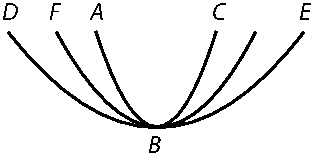
\includegraphics[width=0.33\textwidth]{gesamttex/edit_VIII,3/images/LH_35_09_16_004_d1.pdf}}% \hspace*{16mm}
  \vspace{0.5em}
  \centerline{\lbrack\textit{Fig.~1}\rbrack}% \hspace*{16mm}
  \label{LH_35_09_16_004r_Fig.1}%
\newpage
\pstart
\noindent
 \textit{même vers \textit{E} que si on} auroit \textit{mis un plus petit corps} vers \textit{A}.
\textit{Supposons donc
que le corps Elastique\protect\index{Sachverzeichnis}{corps élastique}
se peut estendre deux pieds,\protect\index{Sachverzeichnis}{pied}
si ont met d'un costé et d'autre des corps egaux,
il s'étendra d'un pied\protect\index{Sachverzeichnis}{pied} de chaque costé.
Que si on met vers \textit{A} un corps double de celuy
qu'on}
\edtext{\lbrack\textit{luy}\rbrack}{%
\lemma{\textit{luy}}\Bfootnote{%
\textit{erg. Hrsg. nach Vorlage}}}
%
\textit{presente en C,
il ne s'etend que} d'\textit{un demy pied vers F,}
\edtext{\lbrack\textit{donc}\rbrack}{%
\lemma{\textit{donc}}\Bfootnote{\textit{erg. Hrsg. nach Vorlage}}}
%
\textit{il aura encor la force de pousser vers E}\lbrack;\rbrack\
\textit{que si le corps en A se trouve immobile,
il s'etendra deux pieds vers E.}\edlabel{LH35_09_16_004r_10}
\pend% Kein Absatz im Text
  \vspace{2.0em}
  \centerline{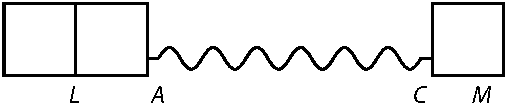
\includegraphics[width=0.54\textwidth]{gesamttex/edit_VIII,3/images/LH_35_09_16_004_d2.pdf}}% \hspace*{16mm}
  \vspace{0.5em}
  \centerline{\lbrack\textit{Fig.~2}\rbrack}% \hspace*{16mm}
  \label{LH_35_09_16_004r_Fig.2}%%
%
\vspace{1.5em}
\pstart%
(\protect\vphantom)+~%
Haec ratiocinatio\protect\index{Sachverzeichnis}{ratiocinatio} satis solida et clara non est.
Malim rem sic concipere. 
% \pend% Kein Absatz im Text
%
%
% \pstart%
\edtext{Elaterium\protect\index{Sachverzeichnis}{elaterium} \textit{AC}}{%
\lemma{Elaterium \textit{AC}}\Cfootnote{%
Siehe das Diagramm \lbrack\textit{Fig.~2}\rbrack.}}
%
quaeritur
an impellat tantum corpus \textit{M},\protect\index{Sachverzeichnis}{corpus impulsum} levius,
an utrumque tam \textit{L} et \textit{M}, et qua ratione.
Si soli \textit{M}
tunc non ita cito restituitur,\protect\index{Sachverzeichnis}{restitutio elaterii}
quam si eodem tempore utrique,\protect\index{Sachverzeichnis}{tempus restitutionis}
licet \textit{L} moveatur tardius quam \textit{M},
itaque utrique imprimitur impetus.\protect\index{Sachverzeichnis}{impetus impressus}
Sed qua proportione?
Respondeo ea qua fit
\edtext{ut elaterium}{%
\lemma{ut}\Bfootnote{%
\textit{(1)}~corpus
\textit{(2)}~elaterium%
~\textit{L}}}
%
quam citissime restituatur.\protect\index{Sachverzeichnis}{restitutio elaterii}
\edtext{Sit \textit{LM}}{%
\lemma{Sit \textit{LM}}\Cfootnote{%
Siehe das Diagramm \lbrack\textit{Fig.~4}\rbrack\ auf S.~\pageref{LH_35_09_16_004r_Fig.4}.}}
distantia prima~\textit{a},
\textit{{\scriptsize1}L{\scriptsize2}L} vocetur \textit{dl},
et \textit{{\scriptsize1}M{\scriptsize2}M} vocetur \textit{dm}, %Umgebungsangleichung für . 
et \textit{{\scriptsize1}L{\scriptsize4}L} vel similis vocetur \textit{l},
et \textit{{\scriptsize1}M{\scriptsize4}M} vel similis vocetur \textit{m}.
% \pend% Kein Absatz im Text
%
%
% \pstart%
Est autem semper ratio eadem \textit{{\scriptsize1}L{\scriptsize2}L}
ad \textit{{\scriptsize1}M{\scriptsize2}M},
quae \textit{{\scriptsize2}L{\scriptsize3}L}
ad \textit{{\scriptsize2}M{\scriptsize3}M},
ergo et semper ratio est eadem \textit{l} ad \textit{m}.
Datur et tota
\edtext{\textit{{\scriptsize4}L{\scriptsize4}M} aequ. \textit{b} aequ. $a + l + m$.}{%
\lemma{\textit{{\scriptsize4}L{\scriptsize4}M}}\Bfootnote{% 
\hspace{-0,5mm}aequ. \textit{b}~%
\textbar\ ergo \textit{gestr.}~%
\textbar\ aequ. $a + l + m$.%
~\textit{L}}}
%
Ut autem investigemus proportionem \textit{m} ad \textit{l},
temporis jam consideratione\protect\index{Sachverzeichnis}{consideratio} opus est.
\edtext{}{%
{\xxref{LH_35_09_16_004r_ adhfbic-1}{LH_35_09_16_004r_ adhfbic-2}}%
\lemma{Elaterium \lbrack....\rbrack\ in \textit{{\scriptsize2}M}}\Cfootnote{%
Siehe das Diagramm \lbrack\textit{Fig.~3}\rbrack\ auf S.~\pageref{LH_35_09_16_004r_Fig.3}.}}%
\edtext{\edlabel{LH_35_09_16_004r_ adhfbic-1}%
Elaterium\protect\index{Sachverzeichnis}{elaterium}
quo tempore\protect\index{Sachverzeichnis}{tempus restitutionis} pellit mobile\protect\index{Sachverzeichnis}{mobile}}{%
\lemma{Elaterium}\Bfootnote{%
\textit{(1)}~semper eodem tempore pellit mo
\textit{(2)}~quo tempore pellit mobile%
~\textit{L}}}
%
\textit{L} in \textit{{\scriptsize2}L},
eo pellit mobile\protect\index{Sachverzeichnis}{mobile} \textit{M} in \textit{{\scriptsize2}M}.%
\edlabel{LH_35_09_16_004r_ adhfbic-2}
\edtext{Imo dubitatur an \lbrack non\rbrack\ semper \lbrack sit\rbrack\ eadem ratio}{%
\lemma{Imo}\Bfootnote{%
\textit{(1)}~videtur non
\textit{(2)}~dubitatur an
\textbar~non \textit{erg. Hrsg.}~%
\textbar\ semper
\textbar~esse \textit{ändert Hrsg.}~%
\textbar\ eadem ratio%
~\textit{L}}}
%
etsi idem semper determinandi principium.
Haec accurate excutienda.
Area \textit{{\scriptsize1}T{\scriptsize4}T{\scriptsize4}L{\scriptsize1}T}
semper debet esse eadem,
nam repraesentat spatium\protect\index{Sachverzeichnis}{spatium extensionis}
in quod se extendit elaterium.%
\protect\index{Sachverzeichnis}{elaterium}\protect\index{Sachverzeichnis}{extensio elaterii}
\textit{TM}, \textit{ML} repraesentant spatiorum incrementa cujusque mobilis.
Suppono semper quadrata celeritatum\protect\index{Sachverzeichnis}{quadratum celeritatis} ambobus
\edtext{corporibus simul impressarum}{%
\lemma{corporibus}\Bfootnote{%
\textit{(1)}~impressarum
\textit{(2)}~simul impressarum%
~\textit{L}}}
%
esse ut spatia percursa:\protect\index{Sachverzeichnis}{spatium percursum}
Rem\edlabel{LH_35_09_16_004r_hsisgh-1}
\edtext{alias}{%
\lemma{alias}\Cfootnote{%
Anspielung nicht aufgelöst.}}
% Möglicherweise in späteren Texten aus diesem Band wie etwa N.~??A29, N.~??A28 \textit{De vi elastica ad rationes geometricas revocata} und N.~??A34 \textit{De motu elaterii se restituentis}.
% ??A18 (De restitutionis potentia) ???
investigabo.\edlabel{LH_35_09_16_004r_hsisgh-2}%
~+\protect\vphantom()
%
\pend%
%
%
 \vspace{1.2em}
  \centerline{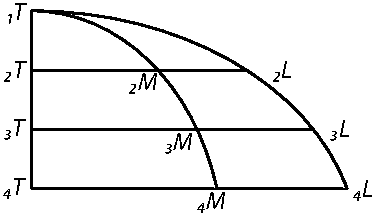
\includegraphics[width=0.38\textwidth]{gesamttex/edit_VIII,3/images/LH_35_09_16_004_d3.pdf}}% \hspace*{16mm}
  \vspace{0.5em}
  \centerline{\lbrack\textit{Fig.~3}\rbrack}% \hspace*{16mm}
  \label{LH_35_09_16_004r_Fig.3}%
%  \vspace*{1.5em}
%
%
  \vspace{2.2em}
  \centerline{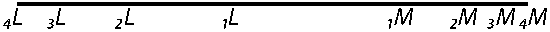
\includegraphics[width=0.56\textwidth]{gesamttex/edit_VIII,3/images/LH_35_09_16_004_d4.pdf}}% \hspace*{16mm}
  \vspace{0.5em}
  \centerline{\lbrack\textit{Fig.~4}\rbrack}% \hspace*{16mm}
  \label{LH_35_09_16_004r_Fig.4}%
  \vspace{1.5em}
%  \newpage%
%
%
 \count\Bfootins=900
 \count\Afootins=1000
 \count\Cfootins=900
\pstart%
[4~v\textsuperscript{o}]
Prop. 6.\protect\index{Sachverzeichnis}{proposition}
\edtext{\textit{Le ressort\protect\index{Sachverzeichnis}{ressort}
partage son action\protect\index{Sachverzeichnis}{action du ressort}
selon la raison reciproque} de la resistence\protect\index{Sachverzeichnis}{resistence}
\textit{des corps},}{%
\lemma{\textit{Le ressort} \lbrack...\rbrack\ \textit{corps}}\Cfootnote{%
\cite{01998}\textsc{Dechales}, \textit{Traitté}, l.~II, prop.~6 (S.~88).% Zitat mit kleiner Abweichung.
}}
%
c'est à dire
prop. 7.\protect\index{Sachverzeichnis}{proposition}
\edtext{\textit{Les quantités de mouvement\protect\index{Sachverzeichnis}{quantité du mouvement}
sont en raison reciproque de} la \textit{resistence}}{%
\lemma{\textit{Les quantités} \lbrack...\rbrack\ \textit{resistence}}\Cfootnote{%
\cite{01998}a.a.O., prop.~7 (S.~90). Zitat mit Auslassung.}}
%
c'est à dire de la pesanteur\protect\index{Sachverzeichnis}{pesanteur} des corps
%
(\protect\vphantom)+~%
ita Chalesius 
\protect\index{Namensregister}{\textso{Dechales} (Chalesius), Claude François Milliet 1621\textendash1678}
noster.
Fatetur
\edtext{alios velle quantitatem motus\protect\index{Sachverzeichnis}{quantitas motus} esse utrobique aequalem.}{%
\lemma{alios \lbrack...\rbrack\ aequalem}\Cfootnote{%
Siehe etwa \textsc{Mariotte}, \textit{De la percussion}, prop.~15 (S.~94\,f.).\cite{00311}
Siehe zudem \textit{LSB} VIII,~2 N.~50, S.~428.9\textendash429.5.\cite{01292}}}
%
\edtext{Inquisitio\protect\index{Sachverzeichnis}{inquisitio} mea rem definiet.}{%
\lemma{Inquisitio \lbrack...\rbrack\ definiet}\Cfootnote{%
Gemeint ist wohl wieder die beabsichtigte Untersuchung, auf die soeben (S.~\refpassage{LH_35_09_16_004r_hsisgh-1}{LH_35_09_16_004r_hsisgh-2}) angespielt wurde.}}
%
Puto tamen
Chalesium\protect\index{Namensregister}{\textso{Dechales} (Chalesius), Claude François Milliet 1621\textendash1678}
errare
quia ex
\edtext{principio meo generali\protect\index{Sachverzeichnis}{principium generale}}{%
\lemma{principio meo generali}\Cfootnote{%
Leibniz spielt wahrscheinlich auf seine \glqq Entdeckung\grqq\ an, dass beim direkten zentralen Stoß zweier sich gleichförmig bewegender Körper die Gesamtsumme der \glqq Kraft\grqq\ $mv^2$ erhalten bleibt.
Aus diesem \glqq allgemeinen Prinzip\grqq, das Leibniz Anfang 1678 in seinen \textit{Schedae de corporum concursu} angekündigt hat (siehe N.~\ref{dcc_08} in diesem Band, S.~\refpassage{LH_37_05_086r_reformatio_idzg-1}{LH_37_05_086r_reformatio_idzg-2}), lassen sich \textendash\ wie hier angedeutet~\textendash\ Mariottes (und Huygens') Theoreme über die Bewegung des gemeinsamen Schwerpunkts bestätigen.
Diesen Theoremen zufolge ruht der gemeinsame Schwerpunkt eben dann, wenn die zwei Körper mit derselben Bewegungsgröße \textit{mv} zusammenstoßen.}}
%
praevideo hoc modo centrum gravitatis\protect\index{Sachverzeichnis}{centrum gravitatis}
\edtext{corporum manere in quiete.%
~+\protect\vphantom()}{%
\lemma{corporum}\Bfootnote{%
\textit{(1)}~tendere semper in eandem plagam eadem celeritate
\textit{(2)}~\textbar~hoc modo \textit{streicht Hrsg.}~\textbar\ manere in quiete.~+\protect\vphantom()%
~\textit{L}}}
\pend%
%
%
\pstart%
\edtext{}{{\xxref{LH35_09_16_004v_1}{LH35_09_16_004v_2}}%
{\lemma{Selon \lbrack...\rbrack\ \textit{balle}}\Cfootnote{%
\cite{01998}\textsc{Dechales}, \textit{Traitté}, l.~II, prop.~7 (S.~91\textendash96, bes. S.~94\,f.).% Resumée mit kurzen wörtlichen Übernahmen.
}}}
%
Selon\edlabel{LH35_09_16_004v_1}
\edtext{ceux qui veuillent que l'effort\protect\index{Sachverzeichnis}{effort} soit egal de deux costés,}{%
\lemma{ceux \lbrack...\rbrack\ costés}\Cfootnote{%
Anspielung auf \textsc{Mariotte}, \textit{De la percussion}, prop.~15 (S.~98\,f.).\cite{00311}
Siehe Leibnizens Auszüge hieraus; \textit{LSB} VIII,~2 N.~50, S.~430.18\textendash431.5.}}
%
il
\edtext{faut que la vistesse\protect\index{Sachverzeichnis}{vitesse}}{%
\lemma{faut}\Bfootnote{%
\hspace{-0,5mm}que
\textit{(1)}~le mouvement
\textit{(2)}~la vistesse%
~\textit{L}}}
%
du boulet\protect\index{Sachverzeichnis}{boulet} et du canon\protect\index{Sachverzeichnis}{canon}
qui recule\protect\index{Sachverzeichnis}{recul du canon}
soyent reciproques contre 
\edtext{\lbrack leurs\rbrack}{%
\lemma{leur}\Bfootnote{%
\textit{L~ändert Hrsg.}}}
%
pesanteurs.
Mais le recul du canon\protect\index{Sachverzeichnis}{recul du canon} fait voir le contraire.
Si deux canons sont chargés de même,
\textit{le plus riche
\edtext{en metail\protect\index{Sachverzeichnis}{métal}}{%
\lemma{\textit{en}}\Bfootnote{%
\hspace{-0,5mm}\textit{metail}
\textit{erg.~L}}}}
%
poussera la balle\protect\index{Sachverzeichnis}{balle} plus loin.
\textit{Un canon\protect\index{Sachverzeichnis}{canon} qui creve}
ferait \textit{autant d'effet} sur le boulet,\protect\index{Sachverzeichnis}{boulet}
c'est à dire
\textit{tousjours la moitie de la force},\protect\index{Sachverzeichnis}{force du canon}
selon moy la resistence\protect\index{Sachverzeichnis}{resistence} plus grande
du canon\protect\index{Sachverzeichnis}{canon}
\edtext{\lbrack\textit{se reflechit}\rbrack}{%
\lemma{fait}\Bfootnote{%
\hspace{-0,5mm}reflechir
\textit{L~ändert Hrsg. nach Vorlage}}}
%
\textit{sur la balle.}\edlabel{LH35_09_16_004v_2}
\pend%
%
%
\pstart%
Il dit lib. 2. prop. 8.\edlabel{LH_35_09_16_004v_quantitasmotus_vrze-1}
\edtext{\textit{le premier principe\protect\index{Sachverzeichnis}{principe de mecanique} de Mecanique porte que la
puissance\protect\index{Sachverzeichnis}{puissance}
ou moment\protect\index{Sachverzeichnis}{moment}
est egal à la quantité de mouvement.\protect\index{Sachverzeichnis}{quantité du mouvement}\edlabel{LH_35_09_16_004v_quantitasmotus_vrze-2}}}%[S.~97]
{\lemma{\textit{le premier} [...] \textit{mouvement}}\Cfootnote{\cite{01998}\textsc{Dechales}, \textit{Traitté}, l.~II, prop.~8 (S.~97).}}
\pend%
%
%
\pstart%
Lib. 3. \protect\index{Sachverzeichnis}{proposition}prop. 24\textsuperscript{me}.\edlabel{LH_35_09_16_004v_forcedouble_oefugl-1}
\edtext{\textit{La force qui est double\protect\index{Sachverzeichnis}{force double} d'une autre
pousse\protect\index{Sachverzeichnis}{force poussante} en haut un corps à une hauteur quadruple.%
\edlabel{LH_35_09_16_004v_forcedouble_oefugl-2}}}%
{\lemma{\textit{La force} \lbrack...\rbrack\ \textit{quadruple}}\Cfootnote{%
\cite{01998}a.a.O., l.~III, prop.~24 (S.~237). Zitat mit Auslassung.}}
\pend%
%
\pstart%
\edtext{\textit{Si un corps est poussé\protect\index{Sachverzeichnis}{corps poussé}
en haut par une force\protect\index{Sachverzeichnis}{force poussant} qui surpasse la plus grande
qu'il peut acquerir en tombant,\protect\index{Sachverzeichnis}{corps tombant}
il employera plus de temps à descendre qu'à monter.}
Le P. Mersenne\protect\index{Namensregister}{\textso{Mersenne}, Marin 1588\textendash1648}
\textit{a experimenté plusieurs fois qu'une fleche\protect\index{Sachverzeichnis}{fleche}
qui employe\protect\index{Sachverzeichnis}{minute seconde}
\edtext{4 secondes}{%
\lemma{4 secondes}\Cfootnote{%
\textit{trois} nach Dechales und Mersenne.}}
%
à monter en employoit cinq à retomber.}}{%
\lemma{\textit{Si un corps} \lbrack...\rbrack\ \textit{retomber}}\Cfootnote{%
\cite{01998}a.a.O., l.~III, prop.~28 (S.~244). Zitat mit Auslassungen.
Vgl. \cite{01227}M.~\textsc{Mersenne}, \textit{Ballistica}, prop.~12 (Paris 1644, S.~30).}}
%
(\protect\vphantom)%
Le vent\protect\index{Sachverzeichnis}{vent} souffle par reprises à cause de la condensation de l'air\protect\index{Sachverzeichnis}{condensation de l'air}.%
\lbrack\protect\vphantom()\rbrack\
\pend
 \count\Bfootins=1200
 \count\Afootins=1200
 \count\Cfootins=1200
%
%	%	%	%	ENDE DES STÜCKS AUF BLATT 4v.